\section{はじめに}
近年, コンテナ型仮想化の普及もあり仮想化技術という存在を様々な場面でよく聞くようになりました. しかし, コンテナ型仮想化技術以外の他の仮想化技術というのは中々個人で扱うような技術・ソフトウェアではないこともあり, あまり知られていないことが多かったりします. また, コンテナ型仮想化技術も便利で環境構築が魔法のようなすごい存在といった漠然とした解釈の人もきっと多いはずです. そこでこの章では, 各種仮想化技術の仕組みや特徴について触れながらふわっと仮想化技術について紹介します.

\section{仮想化技術とは}
仮想化技術にはいくつか種類がありますが, この章では計算機資源を抽象化してOSなどに見せるプラットフォーム仮想化のことを指します. 仮想化することで複数の計算機資源を単一に見せたり, 単一の計算機資源を複数に見せることができます. そしてプラットフォーム仮想化を支えるための技術としてシステム仮想機械(VM, Virtual Machine)と呼ばれる計算機資源をエミュレートするソフトウェアが存在します. 仮想機械の実装はハイパーバイザを始めとしていくつか存在します. 例えば仮想専用サーバ(VPS, Virtual Private Server)のようなサービスでは図2.1にように, 物理サーバ上に仮想化OSによって複数の仮想サーバに分割してユーザに各仮想サーバを提供しています.
\begin{figure}[htbp]
    \centering
    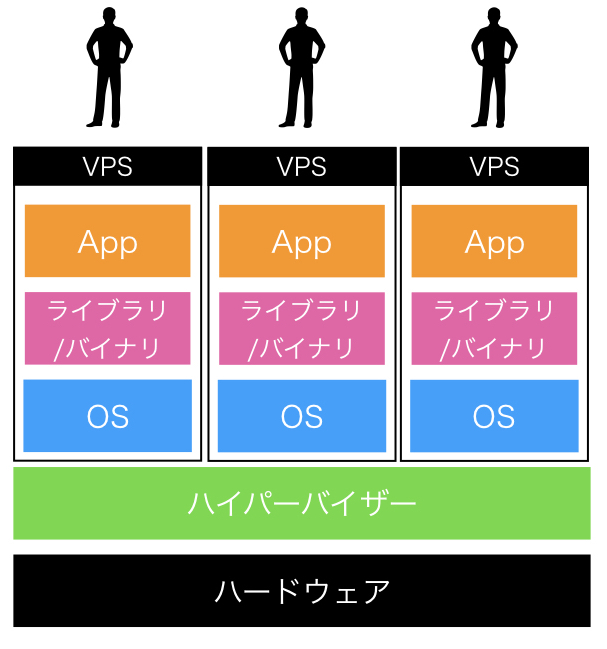
\includegraphics[width=60mm]{./assets/chikuwa_ITasset/vps.jpeg}
    \caption{VPSのイメージ}
    \label{fig:vps}
\end{figure}

\section{ハイパーバイザについて}
仮想化を実現するハイパーバイザにはベアメタル型(Type1),ホスト型(Type2)の2つに分類されます.

\section{ベアメタル型(Type1)}
ベアメタル型(Type1)は, ハードウェアの上で直接動作します. この方式ではホストOSと呼ばれるような土台になるOSが存在しないため,仮想マシンによる遅延や速度低下を防ぐことができます. そしてベアメタルハイパーバイザでは実装手法でもモノリシックカーネル型とマイクロカーネル型の2つに分類することができるほか, 仮想化のアプローチで完全仮想化と準仮想化に分類することができます.
\subsection{モノリシックカーネル型}
主にVMware ESX/ESXiなどで採用されている方式で, モノリシックという英語で「1枚岩」という意味の通り、図2.2のようにハイパーバイザの中にデバイスドライバが含まれています. ハイパーバイザがストレージをはじめ,ネットワークや入力デバイスといったハードウェアへのアクセスをすべてを処理します. この方法の利点はハイパーバイザとデバイスドライバが密接に連携するため,オーバーヘッドが少なく効率的です. しかしながら, ハイパーバイザの中にデバイスドライバが存在しているため,ハイパーバイザ層でデバイスドライバを用意する必要があります. そのため, ハードウェアのサポートがマイクロカーネル型と比較して少なく, 使用するハードウェアに制限がかかってしまう場合があります. また, デバイスドライバをハイパーバイザに直接組み込むため, バグや脆弱性はハイパーバイザ全体に広がってしまいます.
\begin{figure}[htbp]
    \centering
    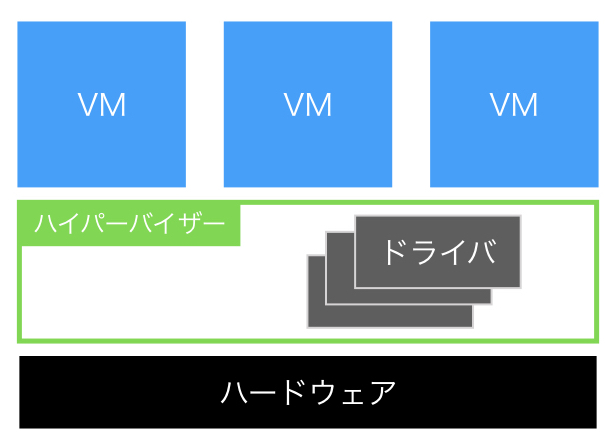
\includegraphics[width=60mm]{./assets/chikuwa_ITasset/monolithic.jpeg}
    \caption{モノリシックカーネル型ベアメタルハイパーバイザ}
    \label{fig:monolithic}
\end{figure}
\subsection{マイクロカーネル型}
主にXenやHyper-Vで採用されている方式で, 図2.3のようにハイパーバイザを管理する仮想マシンと管理OSを用意します. この管理OSはLinuxはWindows Serverなど汎用OSを使用します. また, 管理OSはXenではドメイン0, Hyper-Vでは親パーティションと呼ばれています. この方式では, 図2.4のようにデバイスドライバはハイパーバイザではなく, ハイパーバイザ上の仮想マシンとして動作している管理OSのデバイスドライバを使用します. 仮想マシンからハードウェアにアクセスする時はゲストOSから仮想デバイスのインターフェースを経由してハイパーバイザから管理OSに渡されます. そして管理OSのデバイスドライバからハードウェアにアクセスします.この方法は, 汎用OSのデバイスドライバを使用することで, モノリシックカーネル型に比べてハードウェアのサポートが多く, ハードウェアの対応が柔軟であるという利点があります. 例えば, Hyper-VならWindows用のデバイスドライバを使用することができます. しかしながら, ハードウェアにアクセスする際にハイパーバイザから管理OSを経由するため, モノリシックカーネル型よりも性能が低下してしまいがちであり, 管理用の汎用OSがクラッシュした場合全てのVMがクラッシュしてしまうといった欠点が存在します.
\begin{figure}[htbp]
    \centering
    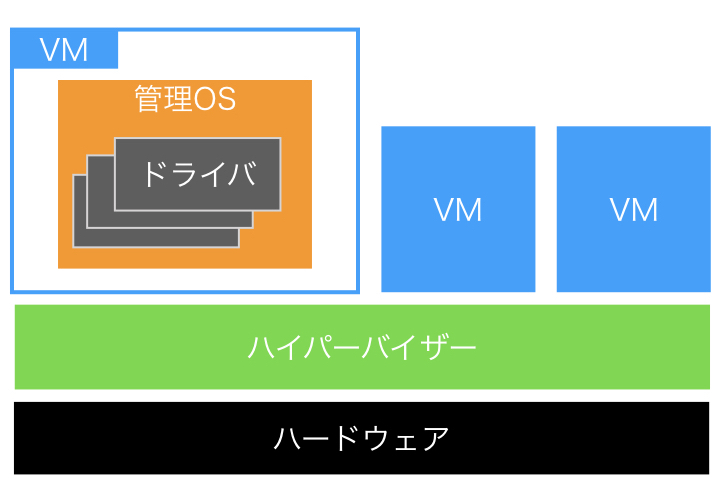
\includegraphics[width=60mm]{./assets/chikuwa_ITasset/microkernel.jpeg}
    \caption{マイクロカーネル型ベアメタルハイパーバイザ}
    \label{fig:microkernel}
\end{figure}
\begin{figure}[htbp]
    \centering
    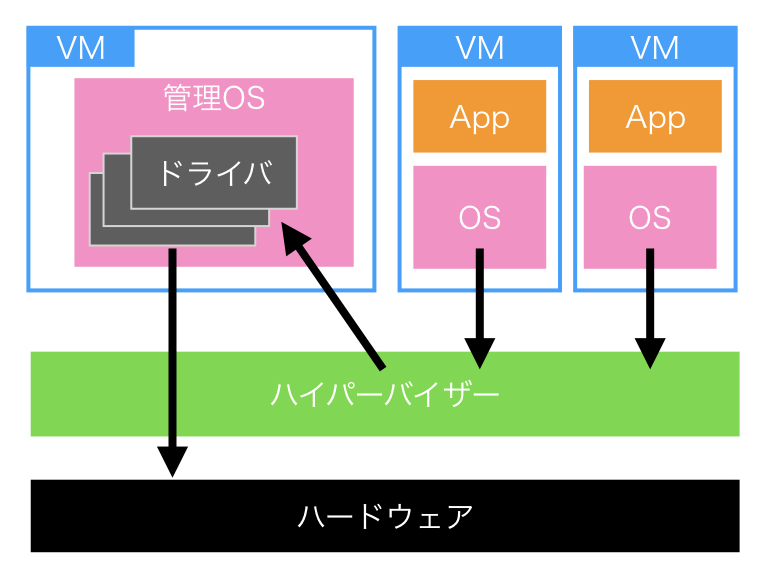
\includegraphics[width=60mm]{./assets/chikuwa_ITasset/microkernel_hardware.jpeg}
    \caption{マイクロカーネル型のハードウェアアクセス}
    \label{fig:microkernel_access}
\end{figure}

\subsection{完全仮想化}
完全仮想化方式のハイパーバイザでは, ハードウェアの挙動をすべてエミュレートします. そのため, 何も変更も加えていないそのままのホストOSを動かすことができます. 1960年代にIBMが「トラップアンドエミュレート」とよばれる方法で完全仮想化を実装しようとしました. この方法ではゲストOSが特権がない状態(Ring3)で実行させ, 特権(Ring0)が必要な命令を実行しようとすると失敗します. その際にハイパーバイザがその失敗をトラップして原因を確認してからその命令をエミュレートすることによってゲストOSの期待する結果を返すことができ, ゲストOSにRing0以外で実行されていることを気づかせないようにすることができます. しかしながら, この手法は古典的ですべてのアーキテクチャに適用できるわけではありませんでした. 特にx86プロセッサの場合, ユーザ権限で実行できるセンシティブ命令と呼ばれる計算機資源の構成などの依存している命令が存在しているため, 実装を難しくさせていました. そこで, 「バイナリトランスレーション」と呼ばれる新しい手法が使われるようになりました. この手法では, センシティブな命令以外の命令は直接CPUで実行し, センシティブな命令はハイパーバイザで実行前に動的に他の命令に置き換えられます.
\begin{figure}[htbp]
    \centering
    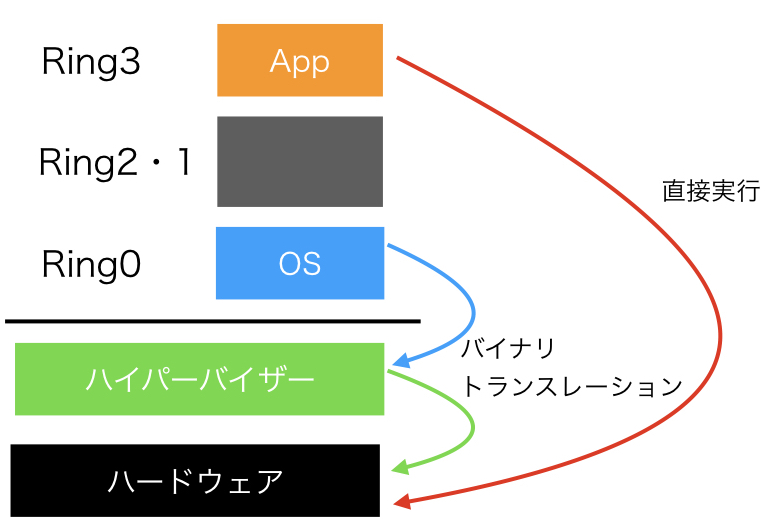
\includegraphics[width=60mm]{./assets/chikuwa_ITasset/binarytransration.jpeg}
    \caption{バイナリトランスレーション}
    \label{fig:binarytranslation}
\end{figure}
\subsection{準仮想化}
準仮想化方式のハイパーバイザでは, ハイパーバイザ上で実行するゲストOSに手を加え, 仮想環境を実現しています. この方式では, ゲストOSのカーネルが発行するハードウェアを制御するシステムコールに手を加えることでハイパーバイザと協調することで高速に動作させようとするものです. なおこのような手を加えられたシステムコールはハイパーバイザコールと呼ばれます. バイナリトランスレーションではセンシティブ命令を動的に変換していたため、性能が低下しやすい特徴がありましたが, 準仮想化では静的に変換を行い修正するため, 性能には影響はありません. しかしながら, ゲストOSに予め変更を加える必要があるため, 使用するゲストOSに制限があるという欠点があります.
\section{ホスト型(Type2)}
ホスト型(Type2)はParallels DesktopやVirtualBoxなどで採用されている方式で, LinuxやWindowsといったホストOSの上でアプリケーションとして動作します. また, ハイパーバイザをインストールする先のPCをホストOSと呼びます. 主にサーバとしての仮想化よりもユーザがmacOS上でWindowsとwindows専用ソフトウェアを使用するといったようなクライアントサイドでの用途に用いられることが多いです. この方式の利点は, ホストOSを変更することもなく, アプリケーションとしてインストールすることができるため手軽に利用することができる点です. 最近ではVargrantのようなプロビジョニングツールが登場したことにより, 手軽に開発環境として仮想環境を用意することができるようにもなりました. しかしながら,ホスト型の欠点として仮想デバイスから物理デバイスにたどり着くまでにハイパーバイザ, ホストOSを経由する必要があるため, オーバヘッドがベアメタル型に比べて大きくなってしまいます.
\begin{figure}[htbp]
    \centering
    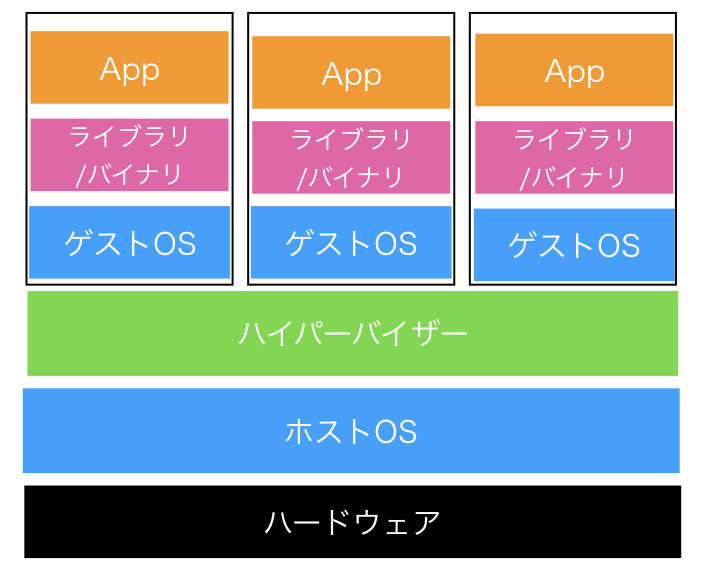
\includegraphics[width=60mm]{./assets/chikuwa_ITasset/host.jpeg}
    \caption{ホスト型ハイパーバイザ}
    \label{fig:hosthypervisor}
\end{figure}
\section{コンテナ型仮想化}
コンテナ型仮想化はハイパーバイザによる仮想化とは少し違う存在で, 単一のOS上に「コンテナ」と呼ばれる仮想的なユーザ空間を提供しています. ここ最近Dockerと呼ばれるコンテナランタイムの普及により注目される存在となってきました. またDocker以外にもLXC/LXDやHaconiwaといった様々なコンテナランタイムが登場しています. これらのコンテナランタイムは一見するとホスト型ハイパーバイザのようにOSの上でOSを簡単に起動しているように錯覚しがちですが, あくまでもコンテナではホストOSの一つの「プロセス」であり,リソースなどを制限したり切り分けていることで一つの小さな独立した環境を作っています. ここからはLinuxコンテナランタイムに焦点を絞り, Linuxのどのような機能を使ってコンテナというものを作り上げていくかを解説していきます.
\section{Linuxコンテナランタイムをつくり上げる技術}
\subsection{chroot}
chrootでは,図のように現在のプロセスとその子プロセスのルートディレクトリを変更します. chroot後の環境から, 別のルートディレクトリや親のファイルシステムを見ることはできません. そのため, chroot監獄とも呼ばれます.しかしながら, chrootした環境内でchrootができる場合, この監獄はすぐに抜けることができてしまうため, 後述するnamespaceやcapabilitiesと併用して安全性を確保します.
\begin{figure}[htbp]
    \centering
    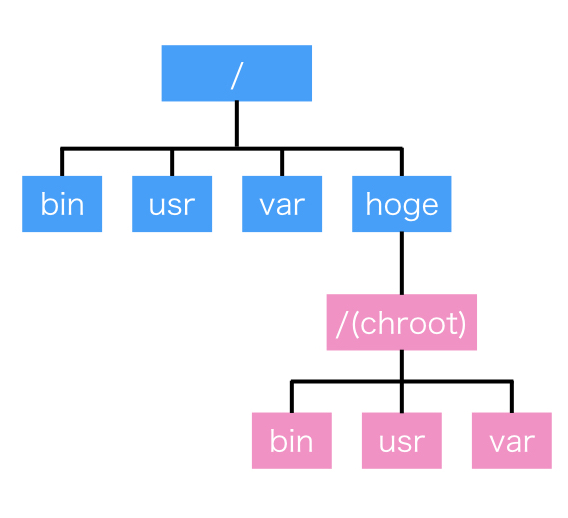
\includegraphics[width=60mm]{./assets/chikuwa_ITasset/chroot.jpeg}
    \caption{chroot}
    \label{fig:chroot}
\end{figure}

\subsection{cgroups}
cgroupsは, プロセスをグループ化してCPUやメモリなどのリソースをコントロールする仕組みです. cgroupsを使うことでCPUのコア数やリソースへのアクセスを再割り当てする一定間隔などを詳細に設定することはもちろん, プロセス数を制限してfork bomb対策をするなどの用途として使用します.
\subsection{Linux namespace}
Linux namespaceはOSのリソースの分離をおこなう仕組みです. Linuxの様々なリソースには「名前空間」と呼ばれるものが存在します. この名前空間を分けてあげることであたかもそのリソースしか存在しないように見せることでリソースを共存させることができます. 今回は4つの名前空間について解説します.
\subsubsection{IPC名前空間}
IPC名前空間はプロセス間通信のリソースであるSystem V IPCオブジェクトとPOSIXメッセージキュー(Linux2.6.30以降)を分離します. IPC名前空間で分離することによって名前空間が異なるプロセスが共有する共有メモリやセマフォにアクセスすることを防ぐことができます.
\subsubsection{Mount名前空間}
Mount名前空間は図のようにファイルシステムのマウントポイントを分離することで異なる名前空間のファイルシステムにアクセスを分離することができます. 通常, 子プロセスは親プロセスと同じマウントポイントを認識します. しかし新しいMount名前空間の下では, 子プロセスは任意の変更を加えることができ,親プロセスやシステム全体のMount名前空間には影響を与えません. 例えば, 各コンテナごとにMount名前空間を分けて/var, /tmpを持たせることで独立したユーザ領域を見せることができます.
\begin{figure}[htbp]
    \centering
    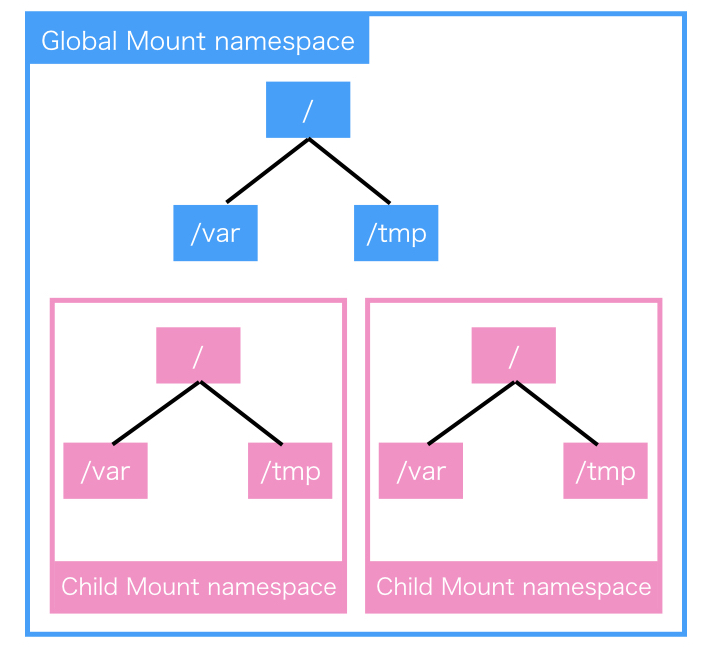
\includegraphics[width=60mm]{./assets/chikuwa_ITasset/mount.jpeg}
    \caption{Mount名前空間}
    \label{fig:mount}
\end{figure}

\subsubsection{PID名前空間}
PID名前空間では, 図のようにプロセスID空間を分離します. 異なるPID名前空間では同じプロセスIDを持つことができ, 子名前空間内のプロセスは親のプロセスについて知ることができません. しかしながら, 親名前空間のプロセスは子名前空間のプロセスについて知ることができます. PID名前空間をコンテナごとに分離することで, コンテナ内のプロセス群を中断再開することやコンテナ内のプロセスのPIDを保持したままコンテナを別のホストに移したりするようなことが可能になります.
\begin{figure}[htbp]
    \centering
    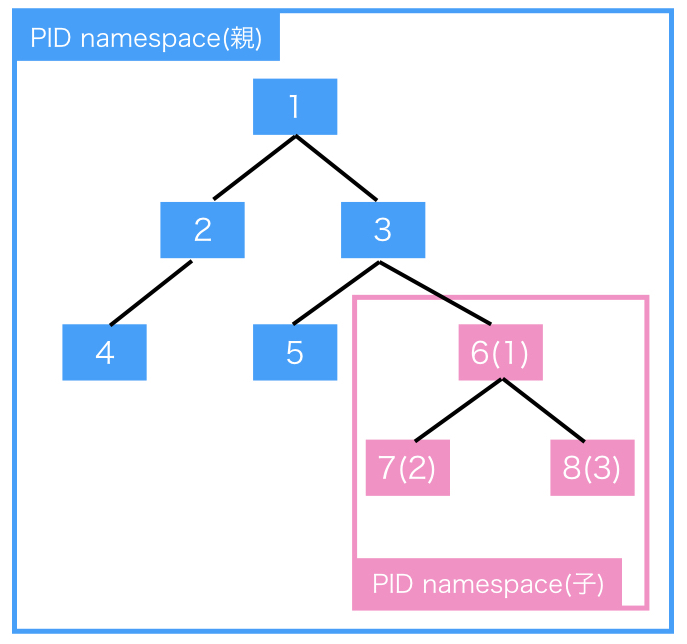
\includegraphics[width=60mm]{./assets/chikuwa_ITasset/pid.jpeg}
    \caption{PID名前空間}
    \label{fig:pid}
\end{figure}

\subsubsection{UTS名前空間}
UTS名前空間では,uname()というシステムコールで返されるホスト名とNISドメイン名を分離します. コンテナでUTS名前空間を分離することによって独自のホスト名とNISドメイン名を設定することができます.
\subsection{capabilities}
Linuxのプロセスには, 特権プロセスと非特権プロセスの2種類が存在します. 例えば, nginxなどのHTTPサーバが1024番ポート未満の特権ポートを使用する際などにプロセスに特権が必要となります. しかし, プロセスにすべての権限を与えてしまうとセキュリティ上あまり良いとは言えず, もっと細分化した権限を与えたい場合があります. そこでLinuxのcapabilitiesでは, 権限をCapabilityと呼ばれる細分化された単位でプロセスに与えることで特権を使用する頻度を下げることができます. capabilitiesは, カーネルのバージョンによって大きく異なりますが/usr/include/linux/capability.h内にある「CAP」からはじまるものがそのカーネルで使うことができるcapabilitiesです. 例えば, CAP\_NET\_BIND\_SERVICEはインターネットドメインの1024番未満の特権ポートをバインドできる権限です. そしてプロセスにはeffective・permitted・inheritableの3種類のケーパビリティ・セットと呼ばれるものがあり, 32ビットのビット列で持っているcapabilitiesを表現しています. effectiveは実際に使用することのできるケーパビリティ・セットで, permittedはプロセスが持つことを許可されているケーパビリティ・セット, inheritableはexecuveの前後で引き継がれるケーパビリティ・セットです.
\section{おわりに}
クラウドやDockerの普及等によってエンジニアにとって仮想化技術というものは当たり前にあるような存在にはなってきましたが, 概念的にも技術的に難しく中々理解したり実装することは難しいですが, ぜひこの機械に普段使っているよう仮想化技術どのようにして出来上がっているのかを見なおしてみると様々なことを知ることができて楽しいはずです。例えば簡単なLinuxコンテナならシェルだけでも出来てしまいますし, 興味があるならぜひやってみると楽しいと思います.
